\chapter{Motivating Example}
\label{ch:Chapter2}
\section{Motivating system: APS}

\begin{figure}
	\centering
	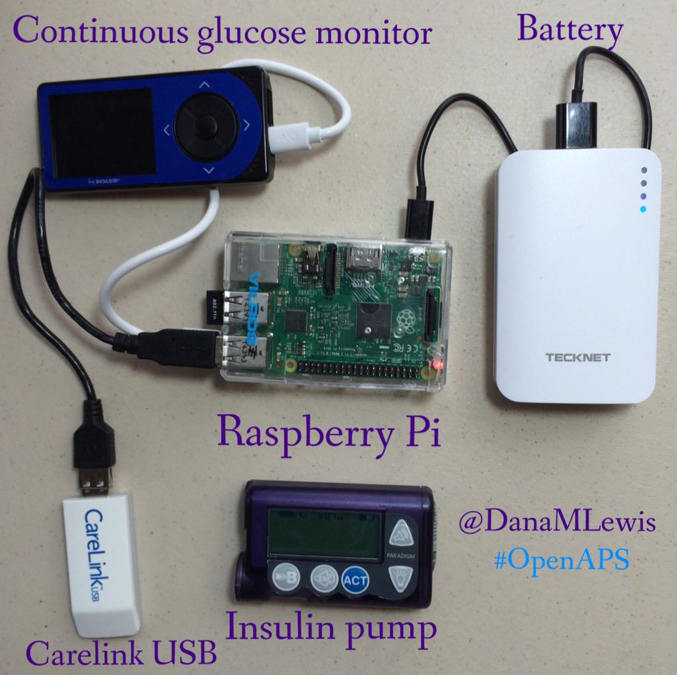
\includegraphics[width=0.7\linewidth]{Images/APSrig}
	\caption{A real world Artifical Pancreas System (APS) Source: openAPS}
	\label{fig:apsrig}
\end{figure}
We use a DNN based Artificial Pancreas system(APS), closed-loop model, by Dutta et al. \cite{10.1007/978-3-319-99429-1_11}  as our motivating example for showing \attack. According to the APS, the patient relies on the model to predict the next dose of insulin to be injected into the body. 


\begin{figure}
	\centering
	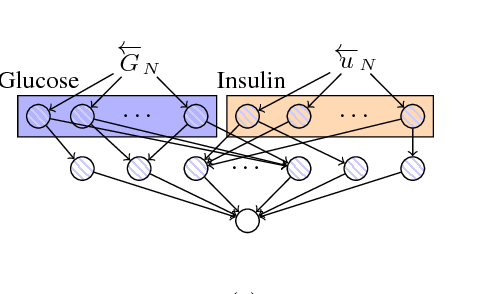
\includegraphics[width=0.7\linewidth, height=0.3\linewidth]{Images/APSDNN}
	\caption[APS DNN]{APS DNN designed by Dutta et. takes in 74 inputs of insulin and glucose. The next layers form connections between the insulin and the glucose to make predictions.}
	\label{fig:apsdnn}
\end{figure}

%How is APS constructed?
The APS consists of sensors and an actuator, one that calculates the blood glucose values and one that injects the insulin inside the body respectively as shown in Figure 3.1. The values from the two sensors are sent to the controller which is the Raspberry Pi in Figure 3.1 which calculates or predicts the next outcome. The network samples the previous blood glucose and insulin values discretized overtime at every 5 minutes. Such a model whose prediction depends on the data collected previously over time is called a data-driven model. The APS DNN model from Dutta et al. is shown in Figure 3.2. The DNN for APS is able to create mappings between the insulin and the glucose values that allow for the prediction of future insulin values. The insulin and the glucose values are the values collected from the sensors and the actuators. The model has 74 inputs in total as shown in Figure 3.2 where 32 inputs are the glucose and the rest are insulin values collected over a span of every 5 minutes. The DNN layers map these values with each other to predict the next value. This basically implies that the future value is predicted based on the inputs from the previous set of values. 


%Defense mechanisms
The APS DNN has certain defense mechanisms accompanying it. The DNN is accompanied by two DNNs that are trained to calculate the upper and the lower bounds to keep a check on the output prediction. In APS there is one output value that implies the outcome for the decision. Initially, expected output value is 140, after the attack the attacker changes it to 190. Due to the accompanying detection mechanisms, the attack will get detected. The range of acceptable output should be between 120-160. Hence, the attacker wants to perturb our inputs such that the output value is below 160 but much higher than 140. Hence, identifying the exact inputs to modify and the right amounts of perturbations that will attack the system without getting detected is the motivation of our work. To do so, we design multiple scenarios where the attack starts at a very basic level and goes on till a level of sophistication where we will require our technique to automatically synthesize attacks. 

%This accompanying mechanism ensures that if the output value was supposed to be 140, does not change to 190 due to some malicious means. If the values don't lie within the bounds alarms are triggered. Our goal is to attack the system within these bounds and still cause some damage. 
%What is our goal
Since APS is a closed-loop system there is no human oversight. Consequently, it is important to ensure that the system is robust against ripples. We discuss a motivating attack below. 


\section{Attack Model}
CPS consist of the physical and the cyber-part. The physical part consists of components such as sensors and actuators. The attacker's goal is to manipulate the sensor measurements to conduct FDIAs without triggering alarms as shown in Figure 3.3. The attacker can use network noise or physical means of sensor tampering to attack the systems. 
The attack is conducted in a stealthy way such that the compromised inputs lie within the threshold ranges. 
%Based on our motivating example of APS, perturbing the inputs slightly and causing ripples ensures that no alarms are triggered. This leads to the wrong prediction of the outputs. However, since the deviation is so small, it is not observable in a closed-loop system by inbuilt error-detection mechanisms. 
\begin{figure}
	\centering
	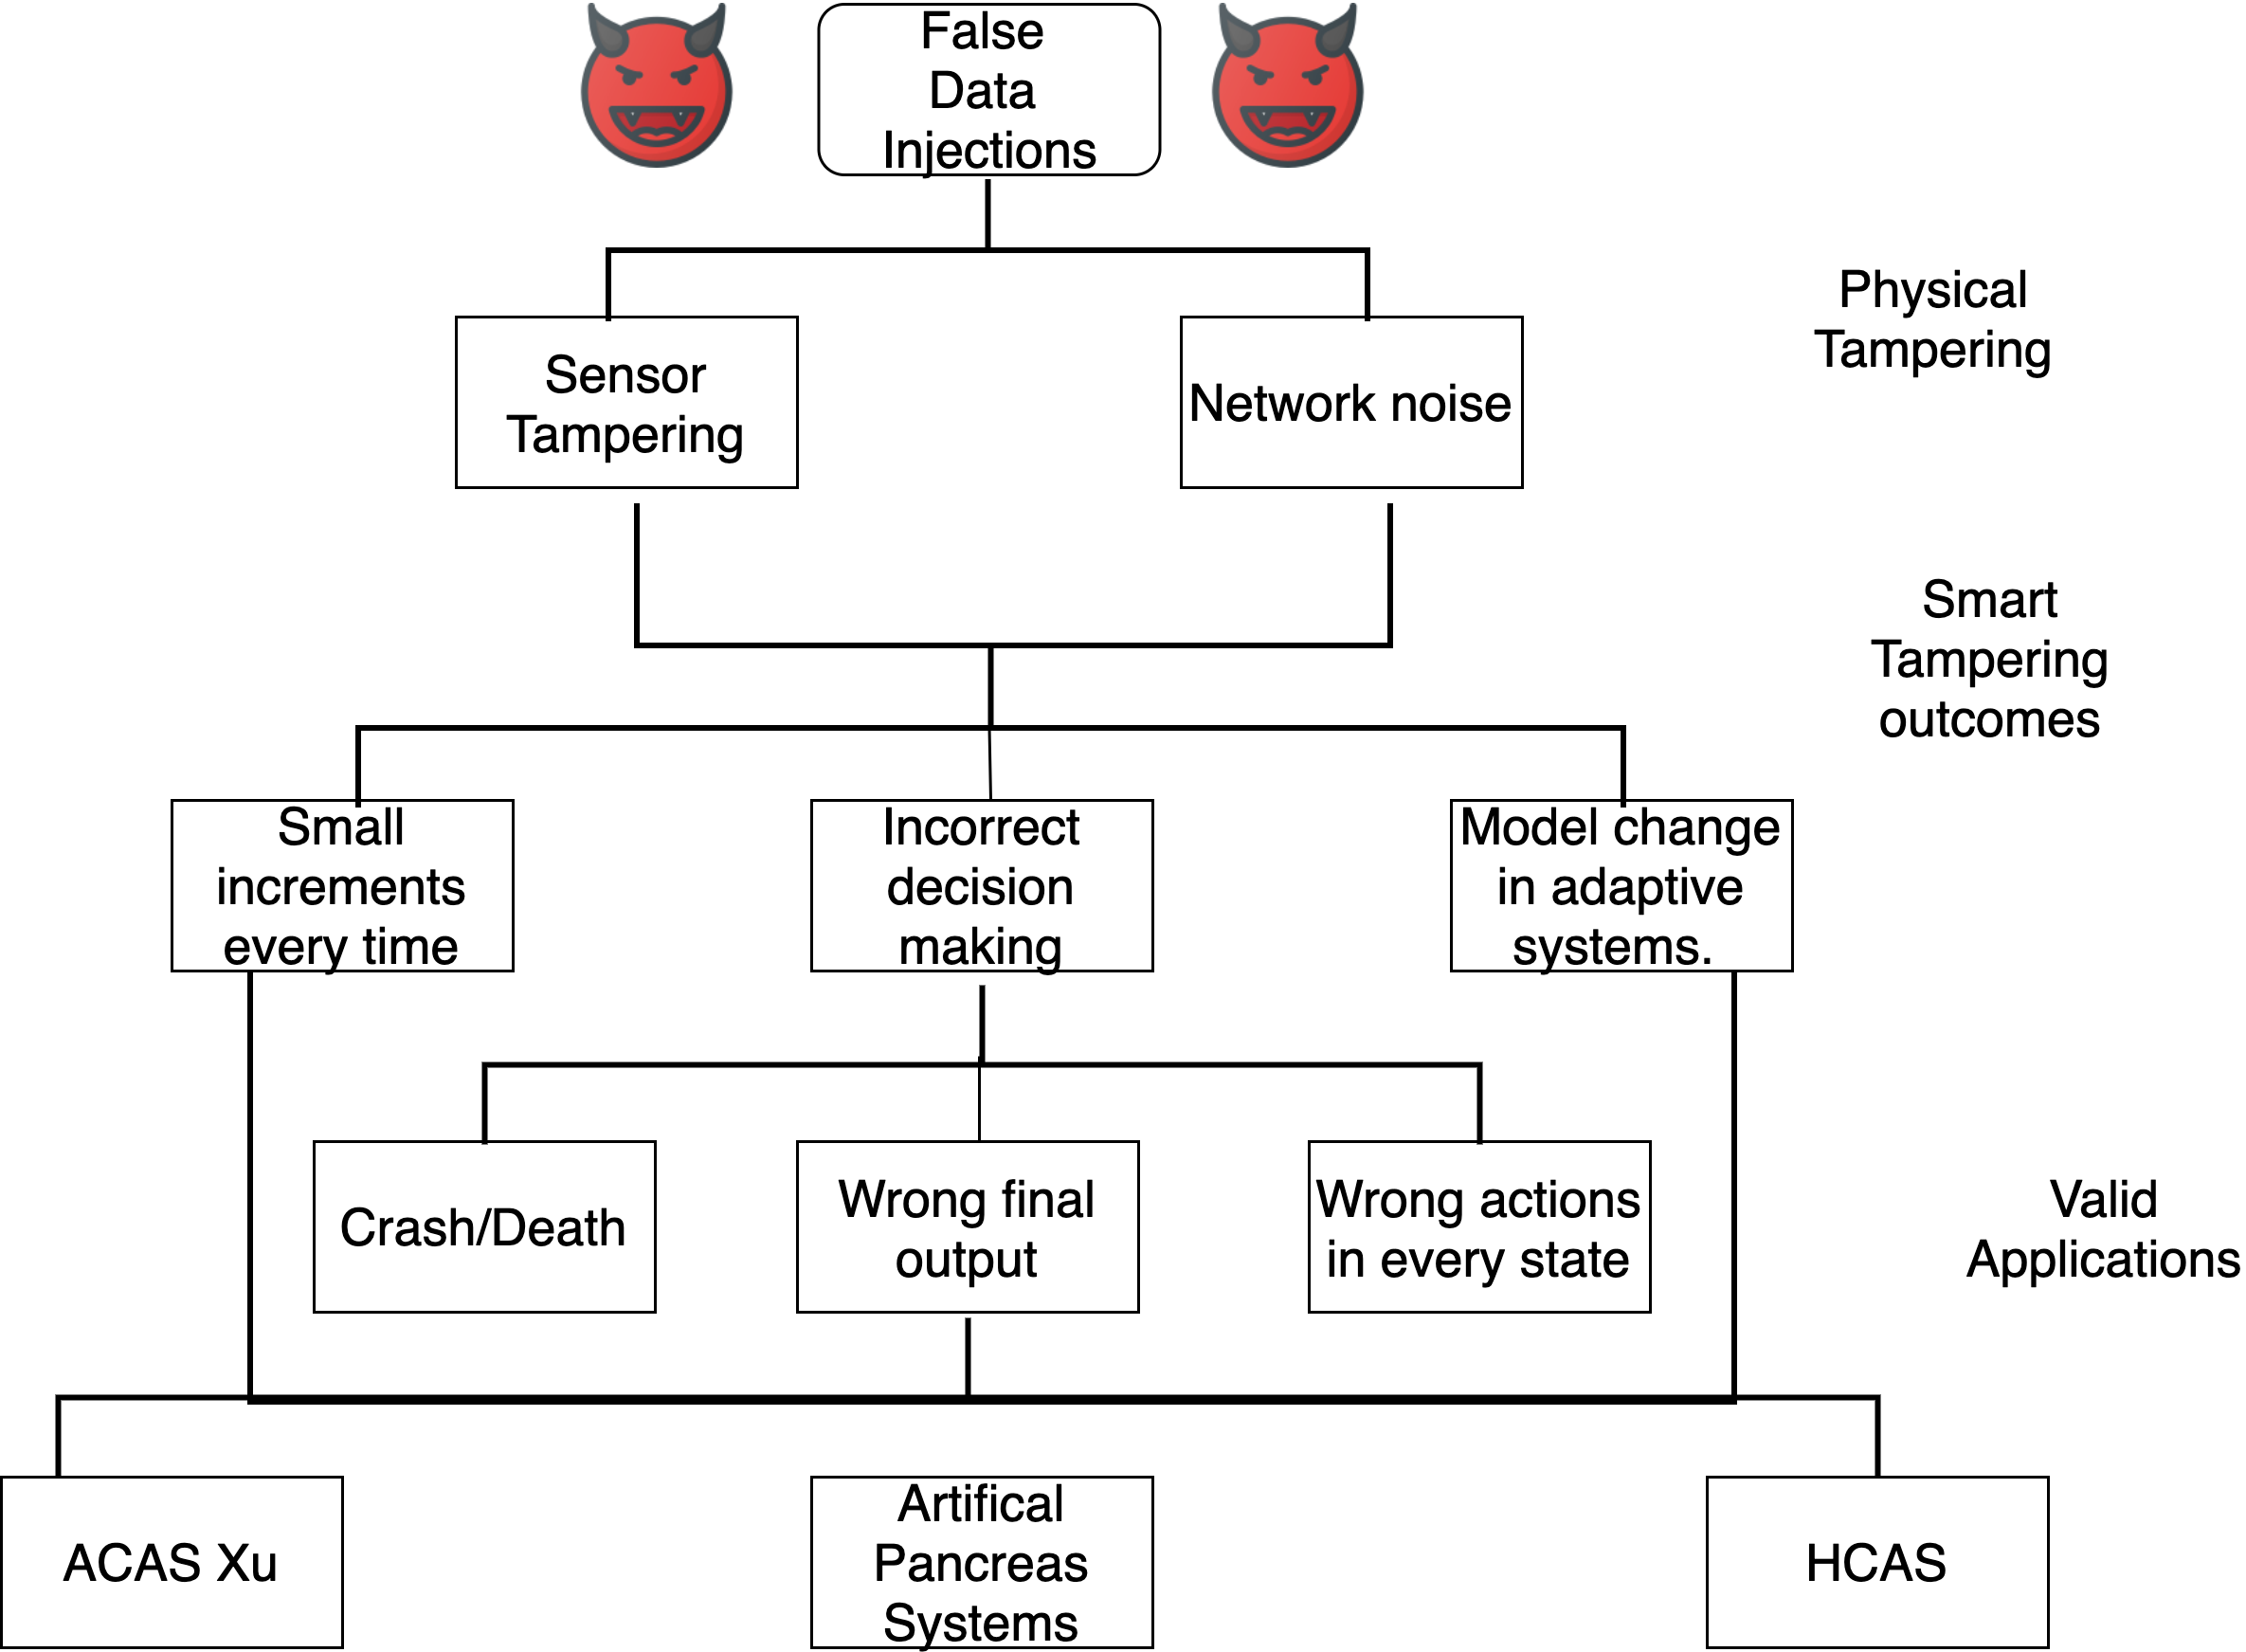
\includegraphics[width=0.7\linewidth]{Images/Attackmodelphysical}
	\caption{Attack model}
	\label{fig:attackmodelphysical}
\end{figure}

We assume that the attacker has following capabilities:
\begin{enumerate}
	\item The weights and bias for the DNN are available through read-only access. There are two parts to obtain the information required for constructing the attacks
	\begin{enumerate}
		\item The architecture of the DNNs
		\item The weights and the bias for the DNNs which are available after the training of the DNN
	\end{enumerate}
We can obtain the above values through the following means
\begin{enumerate}
	\item The DNN architecture can be available from the open-source specfication documents that exist. There are multiple models that are open-source such as openAPS \cite{openAPS}. This provides the attacker the architecture model. For eg. from the openAPS specification document the attacker can infer that developers are using  logistic regression to model the system.  
	There are multiple reverse-engineering mechanisms \cite{10.1145/3195970.3196105} that allows one to infer the DNN models.  
	\item Has one-time access to the system to CPS since the attacker cannot keep injecting false data every five minutes (the data is collected from sensors as explained in the Motivating example section).
\end{enumerate}
  
	%\item Can tamper \smi{add 'with' here} only the physical parts of the CPS such as the sensors based on her targeted attack. 
	\item The attacker does not modify the code but only the inputs to the model.
\end{enumerate}

\subsection{Dumb attacker}
The first way to attack the system would be to change all the 74 values that are the inputs to the DNN. If all the inputs are changed, the final output prediction is going to be wrong. The problem in this particular scenario is that these inputs are collected every five minutes from the sensors attached to the patient as explained above. This means that the attacker will have to conduct false data injection every five minutes when the data is being collected to cause a change in the output. Doing this is not feasible in a practical scenario and hence, the attacker needs a better way of attacking the system. 

\subsection{Smart Attacker}
A more sophisticated approach for the attacker to attack the system would be by perturbing one or two inputs out of the 74 inputs that cause a change in the output. There are two ways to proceed when the attacker tries to change just one or two inputs at a time. 

\subsubsection{Attack 1}
The attacker can randomly choose two inputs and perturb them by huge amounts. This will indeed cause a wrong output prediction. However, if the input is perturbed by very large amounts, the error detection mechanisms will recognize that there is an anomaly. To prevent this the attacker can choose to perturb the two inputs by small amounts. However, perturbing any two random inputs by very small amounts might not necessarily lead to a wrong output prediction.

\subsubsection{Attack 2}
Adding one more layer of sophistication, the attacker supposedly knows the critical inputs or the inputs that on perturbing can lead to wrong predictions. This will be a more targeted approach for attacking the system since the input selection will not be random. Here not knowing the precise amounts by which the critical inputs should be perturbed can lead to an unsuccessful attack. If the perturbation is too high it will trigger the error-detection mechanisms and if it is too low then it will not affect the output. 
\subsubsection{Attack 3}
The most sophisticated means for an attacker to attack the system would be to know precisely which inputs to perturb and by what amounts such that the output prediction is wrong. To do so, the attacker needs an advanced technique that in limited time finds the critical inputs (as we call them) and also the small perturbations that can ensure a wrong output prediction. 

We consider Attack 2c for our evaluation systems and develop a technique called \tool that can automatically synthesize such attacks in a limited amount of time. 



%The attacker does not have write-access to the operating system in the hardware. If the attacker has read-access then she can easily change the code, however, we assume that the attacker can only tamper through physical means.
%We assume that there are error-detection mechanisms that are deployed on top of the APS model that does not allow the attack to be successful if there are huge deviations observed from the input. The final and very important assumption is that the attacker has a limited amount of time to synthesize the attacks and then mount them after the first read access.
%Hence, the attacker needs to find the correct ranges of the inputs to conduct the attack. 





%We use an Artificial Pancreas System(APS) as a running example to motivate the problem and illustrate our technique. This is an example of a safety-critical CPS that uses DNNs.\karthik{Please check}
%A patient using an APS relies completely on the closed-loop model of the APS\cite{10.1007/978-3-319-99429-1_11}. She trusts the model to monitor the body and deliver the right amount of insulin. %However, the APS does not consider side-channel attacks that can be conducted due to the CPS's interface and the presence of DNNs. \karthik{This should be in the Threat model section, not here}
%\karthik{Can you provide a brief description of the APS system, including the role of the DNN? - this is explained in the next paragraph}
%\karthik{You never talk about the DNN through}

%The attackers' goal is to change the inputs slightly such that the amount of insulin to be injected every time is more than the original amount that is supposed to be delivered.
%\karthik{What's the actual amount - the one that is supposed to be delivered when there is no attack}. 
%We want the inputs to be only minutely perturbed such that there is some output deviation observed from the original output. 

%There are two parts to conduct an attack. Since this is a data-driven attack \karthik{What's a data-driven attack? Either cite or define}, 
%the DNN predicts the output by taking in the inputs over time \karthik{What does over time mean?}. Hence, the network has 74 inputs in total \karthik{How does this follow?}. 
%Changing all 74 inputs is not feasible in a practical setting \karthik{What would it entail for the attacker to do this?}. 
%Hence, to conduct a successful ripple attack \karthik{We didn't say the attacker wants to conduct a ripple attack so far}, 
%the attacker needs to first find the critical input and perturb them by specific amounts \karthik{input or inputs}. 
%We provide a technique and automated tool for finding the critical input and further by finding the smallest possible perturbations to those inputs to cause a ripple.
%\karthik{Again, this is already explained in the intro - we need to be specific here} 

%Our proposed synthesized attack can ensure that the inputs are changed in a way that the output always lies within the upper and lower bounds set as constraints for the safety settings for the system. A consistent deviation from the actual value of insulin leads to damage to the patient.  \cite{ZHANG2019403}.

%\karthik{This section is very poorly written - please rewrite it}
%\aarti{Is it easy to understand this? - This is very important to highlight the importance of this work. - there are three models that are deployed together, hence we have to very carefully craft the attacks. }